\documentclass[11pt,a4paper]{article}

\usepackage[utf8]{inputenc}
\usepackage[T1]{fontenc}
\usepackage[english]{babel} % Endret til engelsk
\usepackage{mathpazo}       % Lagt til Palatino / Mathpazo font
\usepackage[margin=2.7cm]{geometry}
\usepackage{microtype}
\usepackage{tikz}
\usetikzlibrary{positioning,arrows.meta,calc}
\usepackage{hyperref}
\hypersetup{colorlinks=true, linkcolor=black, citecolor=blue!50!black, urlcolor=blue!50!black}

% Music notation in LaTeX: for actual musical examples there are MusiXTeX (low-level),
% lilyglyphs/lyluatex (LilyPond integration) and verovio (MEI -> SVG, outside LaTeX).
% For a memo like this, symbols suffice; full notation will be handled in the article version.

\usepackage[blocks]{authblk} % 'blocks' option stacks them neatly vertically if desired

\title{\bfseries Music Notation as a Closed Multimodal System:\\
\large From Transcription to Global Alignment}

\author{Lars G. Bagøien Johnsen}
\author{Thea Mathilde Tollersrud}
\affil{\small The DH Lab, National Library of Norway}

\date{June 12, 2026 \\[2pt] \small Internal memo -- draft. Context: indexing architecture for digital musicology (the OMR project).}

\begin{document}
\maketitle

\begin{abstract}
\noindent
This memo outlines an architecture for music digitization where the musical score (spatial) and the audio recording (temporal) are treated as a single closed, mutually validating system, rather than as two independent, noisy channels. Recognition is reformulated from sequential guessing to global alignment under absolute boundary conditions, and the exchange format (Humdrum/**kern) emerges as the distillate of the cross-validated spatio-temporal matrix. The memo positions this idea against existing work within score--audio synchronization and multimodal transcription, and outlines the trajectory toward an empirical article.
\end{abstract}

\section{The Paradigmatic Shift: Music vs.\ Language}

Traditional digitization of text (OCR) and speech (ASR) rests on a common assumption: both modalities attempt to infer an underlying, linear \emph{ground truth} -- a sequence of ASCII/Unicode characters. Speech and writing are two parallel, independent paths to the same symbolic goal. What is spoken is often not written down, and vice versa.

In musical workflows at the intersection of \emph{Optical Music Recognition} (OMR) and \emph{Automatic Music Transcription} (AMT), this relationship is fundamentally different, even though our goal is to produce a form of \emph{musical ASCII}, such as Humdrum/**kern \cite{huron2002}.

In classical music, the score is a formal set of instructions, and the recorded audio is the compilation or interpretation of those instructions. Everything on the page is meant to be played, and everything played is found on the page. We refer to this as the \emph{performative contract}. It implies that the temporal (the sound) and the spatial (the ink on the paper) validate each other in a completely different manner than what we observe in natural language when constructing the final digital representation. Note, however, that repetitions—which acoustically extend the temporal signal—will be shortened in notation using repetition symbols. Similarly, for songs, often only the first verse is typeset with musical notes, while subsequent verses contain only text.

\section{The Advantage of the Closed System: Global Alignment}

By treating a work as a self-contained whole -- for example, a musical piece consisting of five minutes of audio and a specific number of notation pages -- the task shifts from sequential guessing to \emph{global alignment}:

\begin{itemize}
  \item The first pixel on the first page corresponds to timestamp 0:00.
  \item The last pixel on the last page corresponds to timestamp 5:00.
  \item The system thus operates within absolute boundaries. Recognition is reduced to a process where the spatial and temporal grids are stretched and aligned against each other until inconsistencies are eliminated.
\end{itemize}

Technically, this corresponds to \emph{global} Dynamic Time Warping (DTW) with fixed endpoints over chroma feature representations, as established in the synchronization literature \cite{muller2021fmp,thomas2012,sync2021}. The novelty lies not in the alignment itself, but in elevating it from a post-processing step to a \emph{boundary condition for the recognition process itself} (cf.\ Section~\ref{sec:related}).

\section{Print Ink and Spectrum as Mutual Grounding}

Since the spatial and temporal domains are bound by the performative contract, they function as orthogonal error-correction mechanisms:

\begin{description}
  \item[Ink corrects audio.] A polyphonic, complex audio passage with heavy reverberation, where instruments bleed into one another, can be disambiguated because the visual score defines exactly which independent voices are moving.
  \item[Audio corrects ink.] A damaged, smudged ink cluster on the page that the OMR engine fails to parse visually can be decoded because the audio's frequency spectrum confirms that a crystal-clear C major chord is being played within that exact time window.
\end{description}

\begin{figure}[ht]
\centering
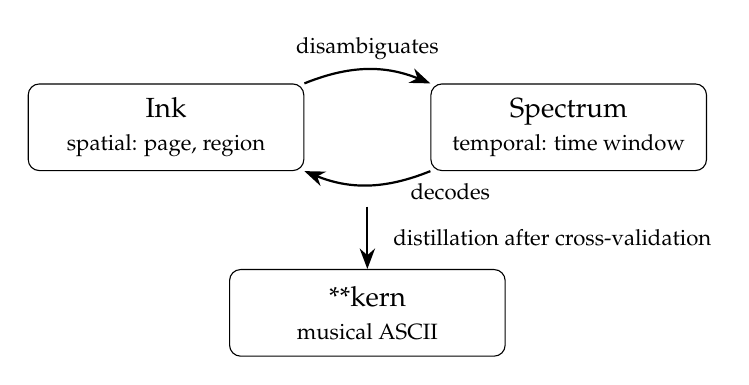
\begin{tikzpicture}[
  node distance=9mm and 16mm,
  boks/.style={draw, rounded corners, align=center, minimum width=35mm, minimum height=11mm},
  pil/.style={-{Stealth[length=2.6mm]}, thick}
]
\node[boks] (sverte) {Ink\\ \footnotesize spatial: page, region};
\node[boks, right=of sverte] (lyd) {Spectrum\\ \footnotesize temporal: time window};
\node[boks, below=18mm of $(sverte)!0.5!(lyd)$] (kern) {**kern\\ \footnotesize musical ASCII};
\draw[pil, bend left=22] (sverte.north east) to node[above, font=\footnotesize]{disambiguates} (lyd.north west);
\draw[pil, bend left=22] (lyd.south west) to node[pos=0.18, below right, font=\footnotesize, inner sep=1pt]{decodes} (sverte.south east);
\draw[pil] ($(sverte.south east)!0.5!(lyd.south west)+(0,-4.5mm)$) -- node[right, font=\footnotesize, xshift=2mm]{distillation after cross-validation} (kern.north);
\end{tikzpicture}
\caption{Mutual grounding: the two modalities stabilize against each other into a cross-validated matrix; **kern is the distillate, not a guess.}
\label{fig:jording}
\end{figure}

\section{The Multimodal Index as a Pathway to **kern}

Instead of relying exclusively on uncertain visual guesses, we allow the image and audio to stabilize against each other into a cross-validated matrix. A position within this system carries coordinates for \emph{both} modalities: a visual region on the score \emph{and} the corresponding acoustic time window.

It is only when this mutual validation is complete that the actual translation occurs. The exchange format distills the entire complex spatio-temporal encounter down to a clean, machine-readable structure. The **kern format (or whichever format we choose; MEI being the alternative with explicit coordinate support) thus assumes its rightful role as musical ASCII -- the final, structured result of the interaction between two modalities.

\section{Related Work and Positioning}
\label{sec:related}

Three research traditions border this proposal. \emph{Score--audio synchronization} \cite{thomas2012,muller2021fmp} established global alignment (OMR $\rightarrow$ chroma $\rightarrow$ DTW $\rightarrow$ coordinates), utilizing fine-grained datasets like MSMD \cite{dorfer2018} and neural alternatives to the OMR+DTW chain \cite{henkel2021}. Audio is used here for \emph{linking and delivery}, not as a corrective mechanism during recognition. \emph{Multimodal transcription} (the Alicante group) \cite{delafuente2022,alfaro2023,alfaro2026} fuses OMR and AMT hypotheses but treats the modalities as parallel, independent channels -- precisely the OCR/ASR model from Section~1 -- finding that the visual modality dominates on clean, modern, and partially synthetic material. \emph{Unified tokenization models} \cite{unified2025} show that joint training on image--audio pairs yields an implicitly shared structure, providing empirical backing for the grounding intuition. Closest in institutional context is CollabScore \cite{rigaux2024}, which builds pivot notation and IIIF linking for cultural heritage collections, but addresses OMR uncertainty via crowdsourcing rather than the acoustic spectrum. For an overview of the OMR field, see \cite{calvozaragoza2020}.

The gap is thus precise: \emph{the closed system as a global boundary condition, using audio as an epistemic corrective within the recognition process itself, applied to historical collection material}. The value of acoustic grounding is not constant -- it grows as image quality degrades and the strength of the contract holds. Existing fusion studies have evaluated it where it is least valuable; a national library's collections are where it is most valuable.

\section{Future Work}

\begin{enumerate}
  \item \textbf{Prototype} (ongoing): Jupyter pipeline utilizing \texttt{music21}, \texttt{librosa}, and global DTW; residuals along the optimal path are aggregated per measure, flagging violations of the performative contract.
  \item \textbf{Bayesian Layer}: a latent node per measure (correct / OMR error / performance deviation / structural break) with ink evidence (OMR confidence) and audio evidence (residual); neighboring measures are chained together, given that structural breaks are spatially correlated while OMR errors occur pointwise.
  \item \textbf{Degradation Experiment}: controlled degradation of scans (blur, smudges, contrast loss), measuring the symbol error rate with and without audio correction as a function of the degradation degree. Hypothesis: the gain from acoustic grounding is a growing function of image degradation; the crossover point is to be determined.
  \item \textbf{Publication}: pending strong results, we target CHR 2027 (Manchester, January 5--8, 2027; submission deadline August 14, 2026) -- a short paper focusing on the framework and prototype, or alternatively, a long paper detailing the degradation experiment.
\end{enumerate}

\bibliographystyle{plain}
\bibliography{referanser}

\end{document}